\documentclass[tikz,border=3mm]{standalone}
\usepackage[utf8]{inputenc}
\usepackage[T1]{fontenc}
\usepackage{helvet}
\renewcommand{\familydefault}{\sfdefault}
\usetikzlibrary{arrows.meta,positioning}
\begin{document}

\tikzset{every node/.append style={font=\sffamily\small}}
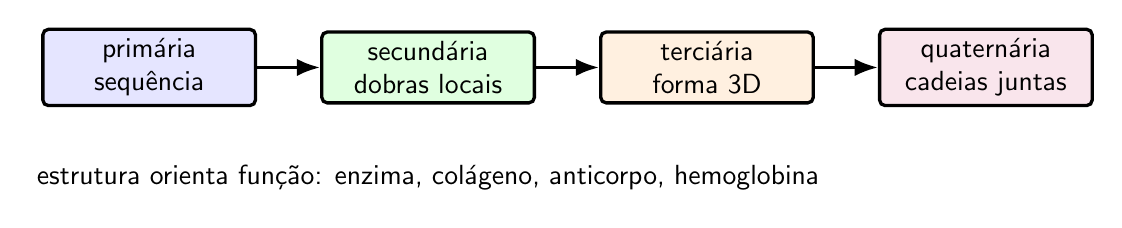
\begin{tikzpicture}[>=Latex,node distance=0.8cm]
  \tikzstyle{box}=[draw,rounded corners=2pt,very thick,align=center,minimum width=2.7cm,minimum height=0.75cm]
  \node[box,fill=blue!10] (p1) {primária\\sequência};
  \node[box,fill=green!12,right=0.8cm of p1] (p2) {secundária\\dobras locais};
  \node[box,fill=orange!12,right=0.8cm of p2] (p3) {terciária\\forma 3D};
  \node[box,fill=purple!10,right=0.8cm of p3] (p4) {quaternária\\cadeias juntas};
  \draw[very thick,->] (p1) -- (p2);
  \draw[very thick,->] (p2) -- (p3);
  \draw[very thick,->] (p3) -- (p4);
  \node[align=center,below=0.65cm of p2] {estrutura orienta função: enzima, colágeno, anticorpo, hemoglobina};
\end{tikzpicture}
\end{document}
